\begin{appendices}
 

\chapter{OSKAR BEAMPATTERN AND FOREGROUND SIMULATIONS} % Main appendix title
\label{appendix:A1}
% \appendix 
\section{Modelled and measured beams}  \label{sec:A}

The Mueller matrix representations in Fig.~\ref{fig:A1} show the  different perturbation methods (i.e. gain, phase and surface orientation errors) used to corrupt the OSKAR beam model. Note that the distortions in Fig.~\ref{fig:A1}, are clearly visible at the upper and lower diagonals of the beams.
These perturbed beams are then compared with the errors produced from \enquote{real} measured beams of the VLA in Fig.~\ref{fig:A2}. % \ContinuedFloat
The PBs presented in Fig.~\ref{fig:A2} are taken from 2 different stations (i.e. antennas $5$ and $6$) whose fractional differences (refer to Fig.~\ref{fig:truosk4}) 
are relatively higher than any other pair of stations.


 \begin{figure}
 \begin{minipage}[!b]{\linewidth}
  \centering
     \begin{subfigure}[b]{0.8\textwidth}
                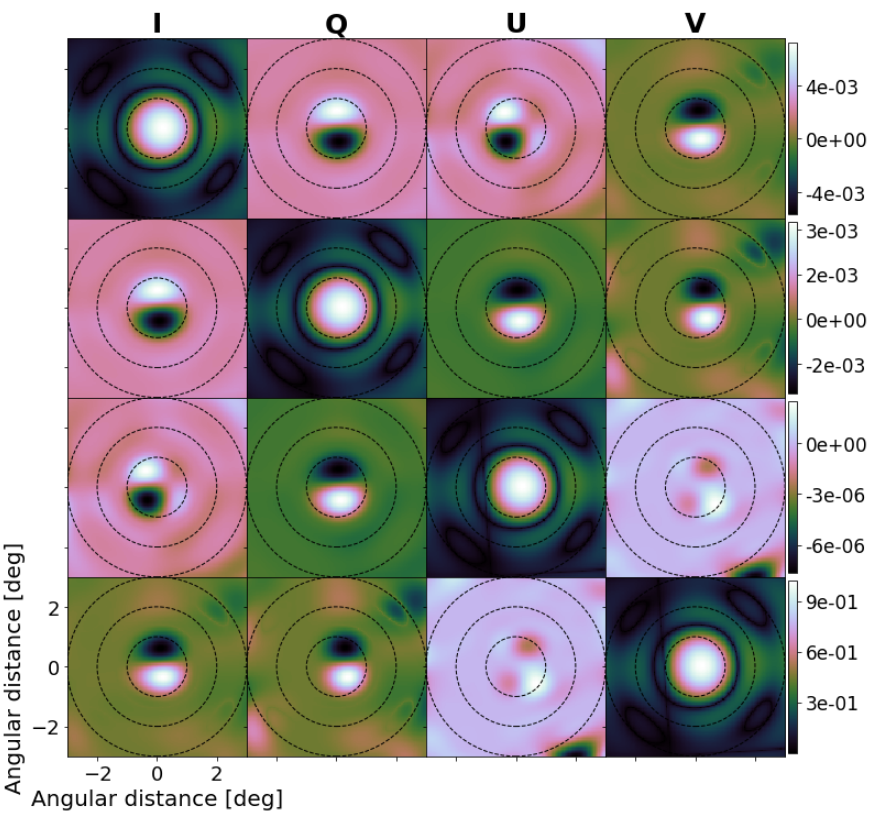
\includegraphics[width=\textwidth]{sec2oskbms/osk_gpmueller}
                \caption{}
                \label{fig:A1a}
        \end{subfigure}
        \begin{subfigure}[b]{0.8\textwidth}
                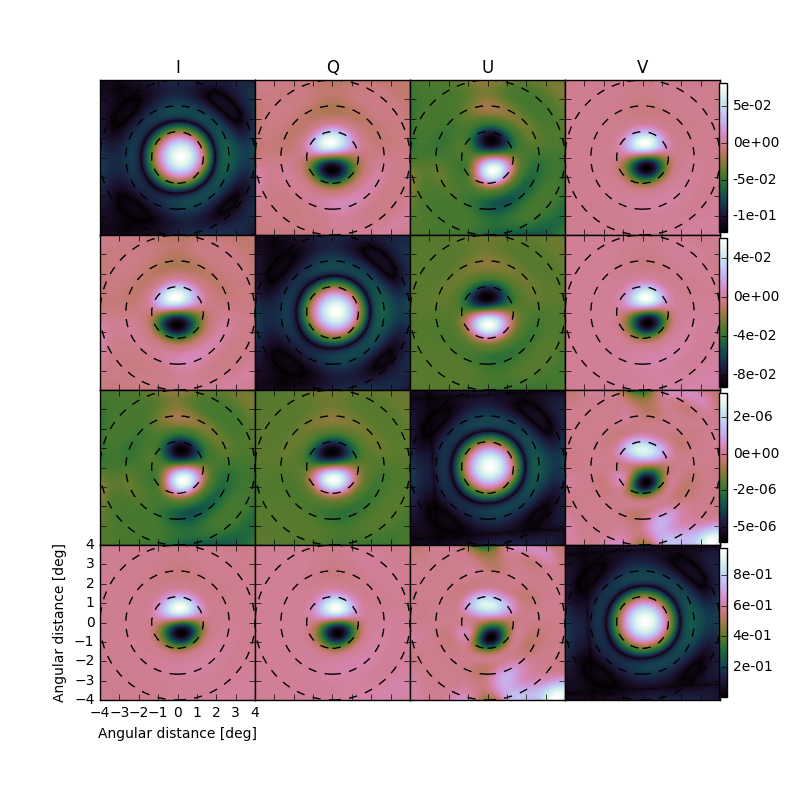
\includegraphics[width=\textwidth]{sec2oskbms/osk_xymueller}
                \caption{}
               \label{fig:A1b}
        \end{subfigure}
         \end{minipage}
        \caption{Fully polarised distorted primary beams of KAT-7. (a) Due to gain and phase errors.  (b) Due to dipole orientation errors.}
	    \label{fig:A1}
  \end{figure}
  \FloatBarrier
 %


\begin{figure}
  \centering
  \begin{minipage}[H]{\linewidth}
     \begin{subfigure}[b]{0.8\textwidth}
                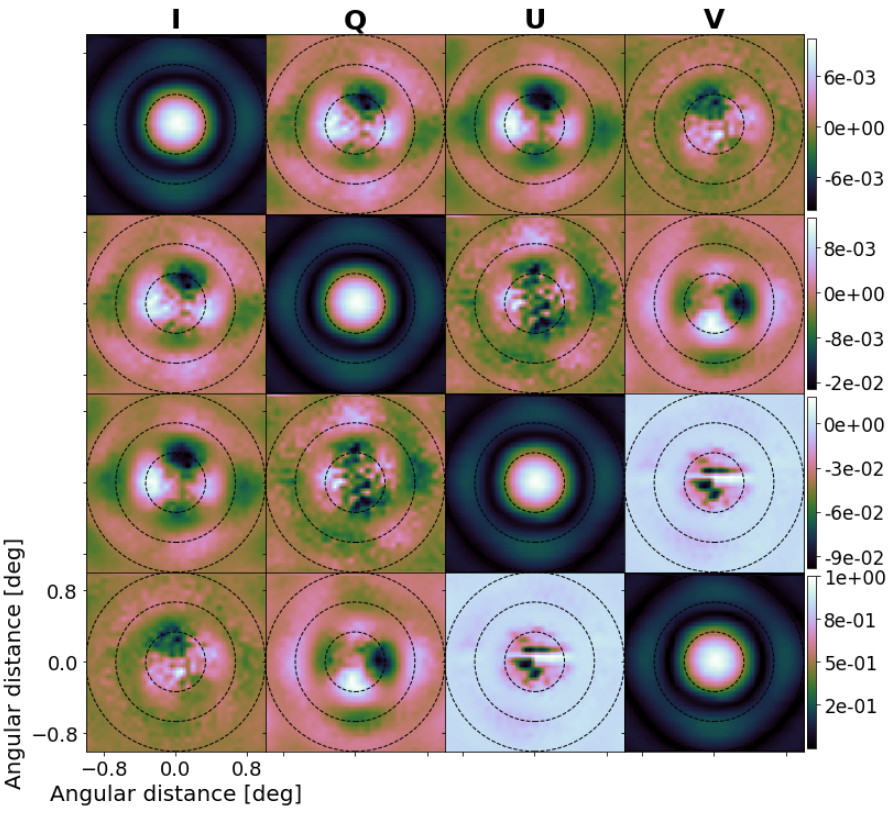
\includegraphics[width=\textwidth]{sec2realbms/vla5mueller}
                \caption{}
                \label{fig:A2a}
        \end{subfigure}
        \begin{subfigure}[b]{0.8\textwidth}
                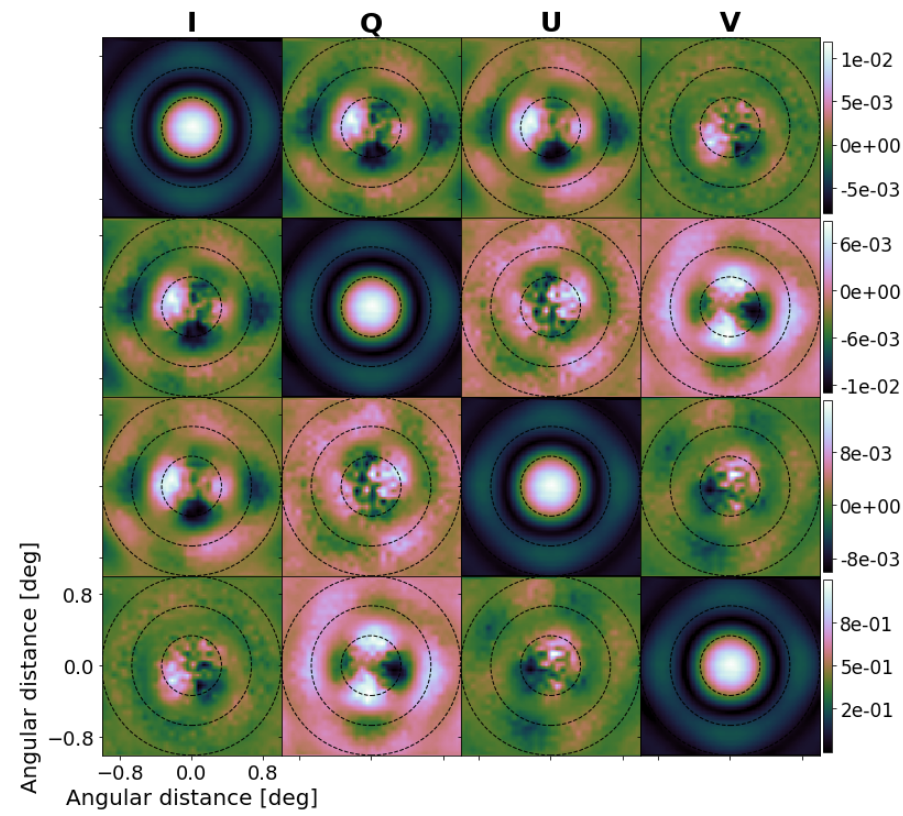
\includegraphics[width=\textwidth]{sec2realbms/vla6mueller}
                \caption{}
               \label{fig:A2b}
        \end{subfigure}
         \end{minipage}
        \caption{$1\, \mathrm{GHz}$ holography measured Mueller beams of VLA. (a) Antenna $5$.
      (b) Antenna 6.} \label{fig:A2}
  \end{figure}
  \FloatBarrier
%%


\section{Measured Full-sky maps} \label{sec:B}
%%
  %	++++++++++++++++++++++++++++++++++++++++++++
%%

% Fig.~\ref{fig:BB1} displays the complete corrupted convolved maps generated from simulating the foregrounds in Fig.~\ref{fig:fg8} with perturbed model beams (due gain and phase errors) in Fig.~\ref{fig:A1a}.

%\begin{quotation}
%\enquote{
Figs.~\ref{fig:B1} and~\ref{fig:B2} represent the respective systematic error maps and the overall full-sky convolved maps simulated with the holography measured beams 
JVLA in Fig.~\ref{fig:A2}. The latter maps are used to produce the convolved power spectrum of the JVLA as presented in Fig.~\ref{fig:fg15}. 
%\indent Table~\ref{tbl:excel-table} displays the errors recorded in the angular power spectrum estimation when modelled beams are assumed, 
%whilst the foregrounds are actually convolved with real measured beams. These errors are tabulated from the absolute differences 
%of the standard errors reported in Fig.~\ref{fig:fg18}.}
%\citep{ansah2018simulations}
%\end{quotation}
%%
%%% +++ RESIDUAL ++++++
%%
 \begin{figure}
\begin{minipage}[H]{\linewidth}
      \centering
      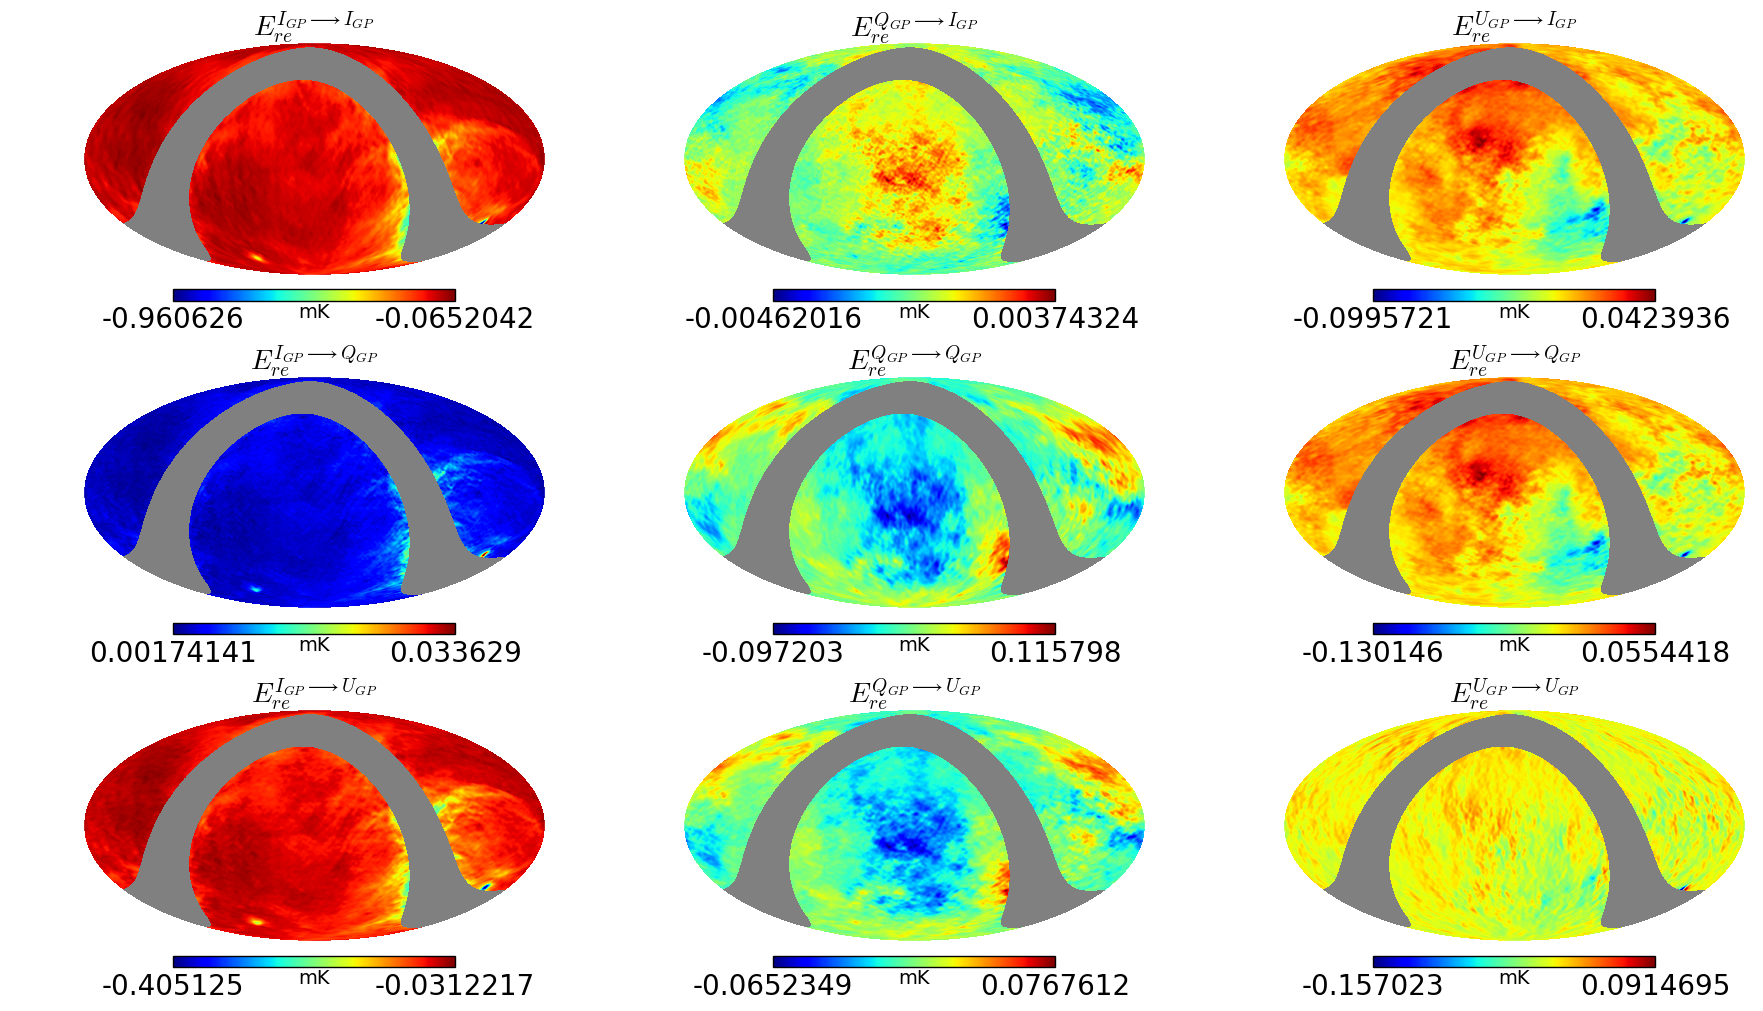
\includegraphics[width=6.6in]{sec3gp_conv/osk_errG1}
      \end{minipage}
 \caption{Systematic errors of full-sky maps produced by computing the relative error between the absolute of the convolved true sky maps and the corrupted sky maps due to gain and phase error beams.}\label{fig:fgerr}
\end{figure}
\FloatBarrier
%%

\begin{figure}
\begin{minipage}[H]{\linewidth}
      \centering
      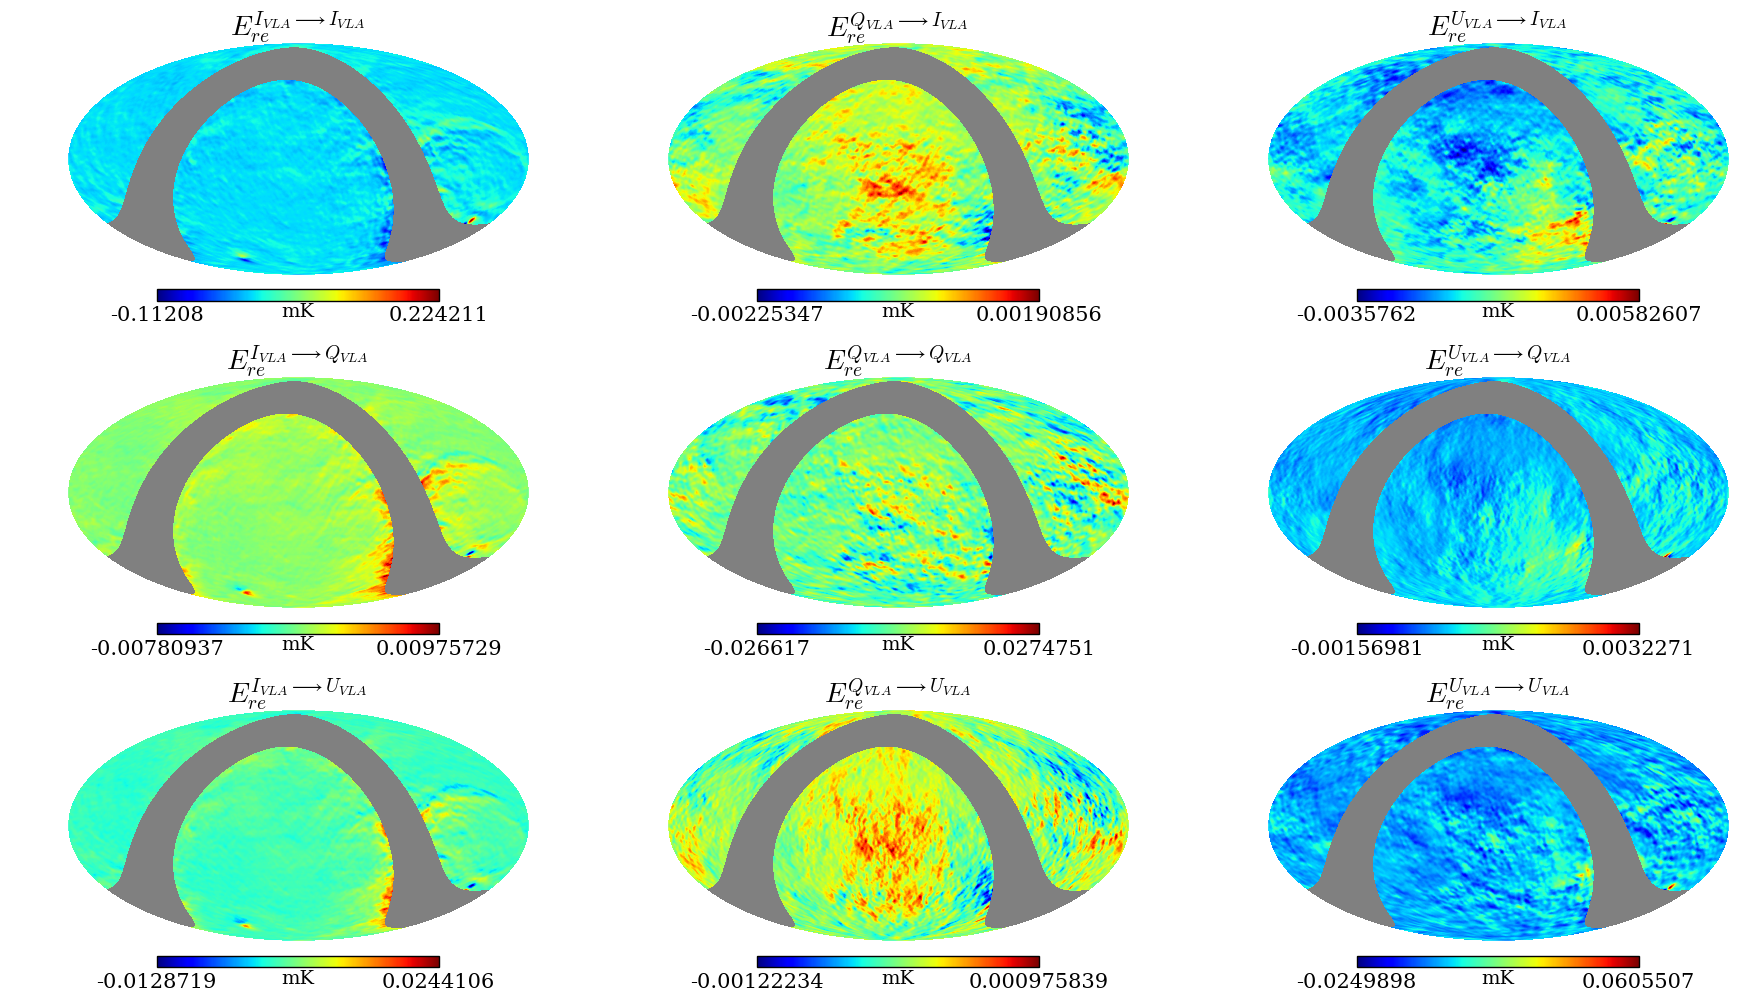
\includegraphics[width=6.6in]{sec3gp_conv/osk_V5-V6_err}
      %xy_All_chan_2}
    \end{minipage}
     \caption{Systematic differences of the full-sky polarisation maps produced by computing the relative error between the convolved sky using VLA PBs in Fig.~\ref{fig:A2}.}  \label{fig:B1}
\end{figure}
    \FloatBarrier
%%% +++ RESIDUAL ++++++
%
%%%%


\begin{figure}
\begin{minipage}[H]{\linewidth}
      \centering
      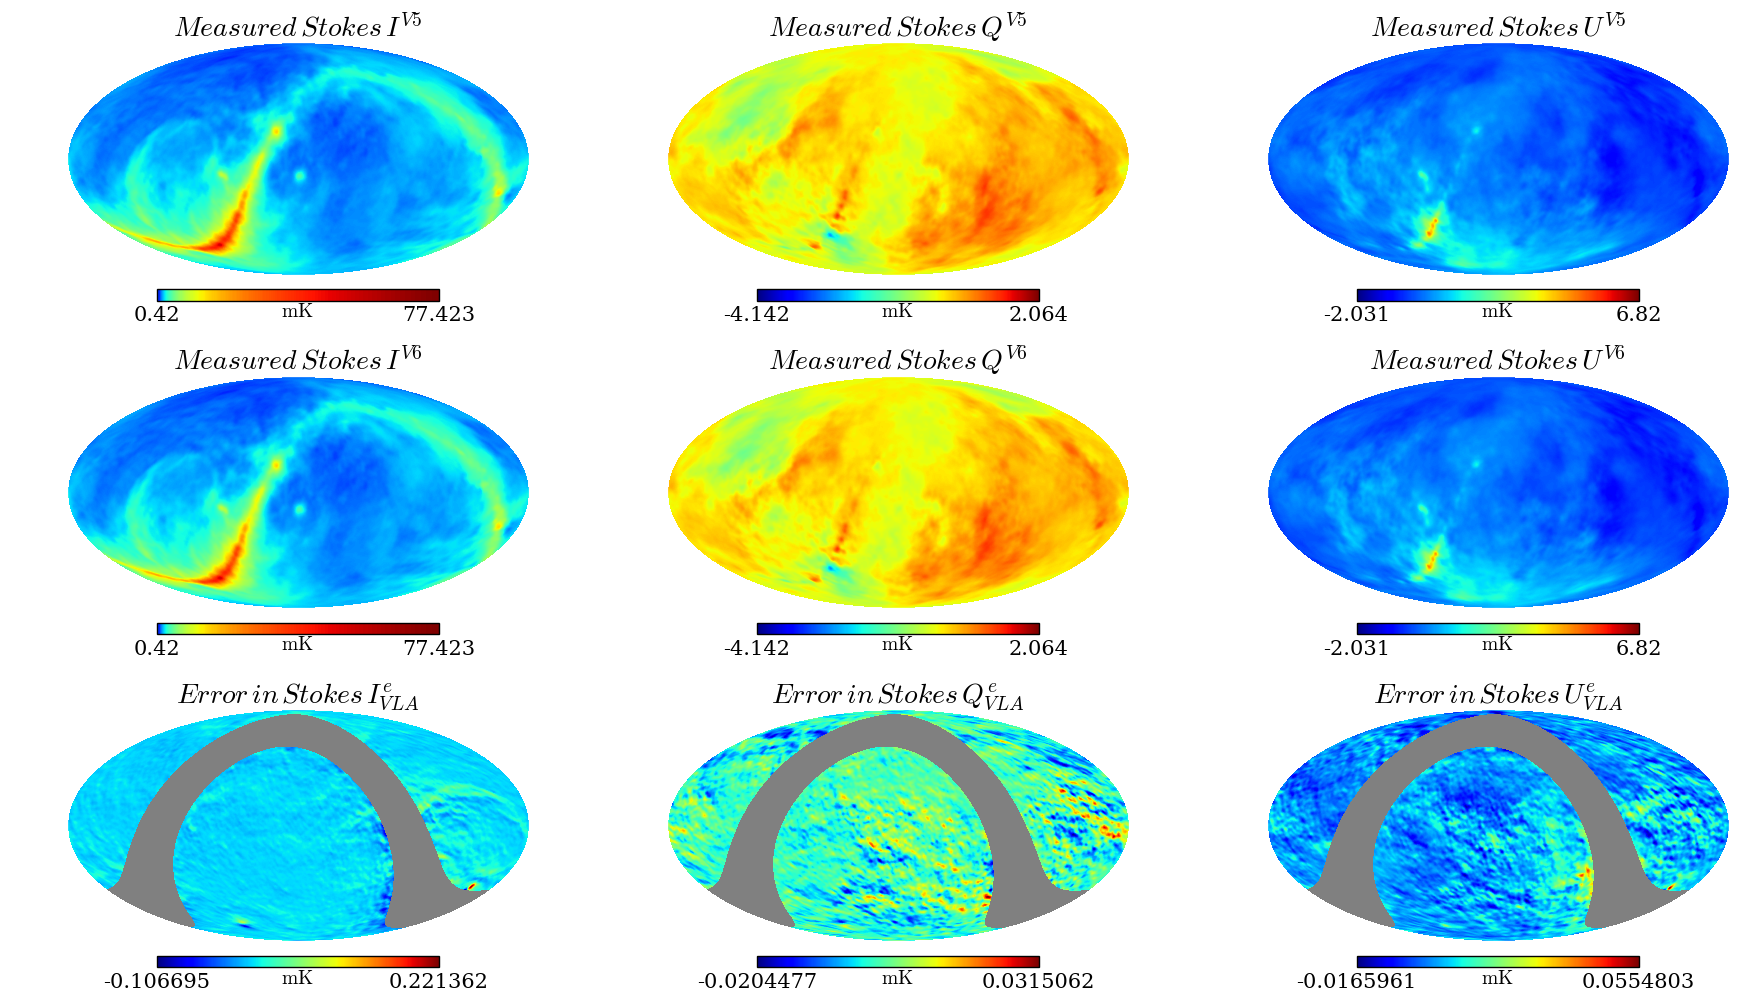
\includegraphics[width=6.6in]{sec3gp_conv/osk_VLA-ALL}
      %v_All_chan_2}
    \end{minipage}
     \caption{Measured Stokes $I$, $Q$ and $U$  for holography measured beams of JVLA with corresponding errors terms.}\label{fig:B2}
    \end{figure}
    \FloatBarrier
    %%
 
 \chapter{Zernike Polynomial Sequence} % Main appendix title
\label{appendix:A2}   
 %%
In this research, we will deal exclusively with the double indexed Zernike polynomials as portrayed by \citet{campbell2003new,lakshminarayanan2011zernike}. 

\begin{table}[H]
% Add the following just after the closing bracket on this line to specify a position for the table on the page: [h], [t], [b] or [p] 
%- these mean: here, top, bottom and on a separate page, respectively
\caption{Relationship between single and double index schemes to third order.} % Table caption, can be commented out if no caption is required
\label{tab:single_index} % A label for referencing this table elsewhere, references are used in text as \ref{label}
\centering % Centers the table on the page, comment out to left-justify
\begin{tabular}{l c c c c c c c} % The final bracket specifies the number of columns in the table along with left and right borders which are specified using vertical bars (|); each column can be left, right or center-justified using l, r or c. To specify a precise width, use p{width}, e.g. p{5cm}
\toprule % Top horizontal line
& \multicolumn{7}{c}{Angular frequency, $m$} \\ % Amalgamating several columns into one cell is done using the \multicolumn command as seen on this line
\cmidrule(l){2-8} % Horizontal line spanning less than the full width of the table - you can add (r) or (l) just before the opening curly bracket to shorten the rule on the left or right side
Radial order, $n$ & -3 & -2 & -1 & 0 & 1 & 2 & 3\\ % Column names row
\midrule % In-table horizontal line
0 &   &   &  & $j=0$ &   &  &  \\ % Content row 1
1 &  &   & $j=1$  &   & $j=2$  &   & \\ % Content row 2
2 &   & $j=3$  &   & $j=4$  &   & $j=5$  & \\ % Content row 3
3 & $j=6$  &   & $j=7$  &  & $j=8$  &   & $j=9$ \\ % Content row 4
% JSB724 & 0.916 & 0.933 & 0.482 & 0.644 & 0.937\\ % Content row 5
\midrule % In-table horizontal line
\midrule % In-table horizontal line
% Average Rate & 0.920 & 0.882 & 0.477 & 0.539 & 0.923 & 0.682 & 0.801\\ % Summary/total row
% \bottomrule % Bottom horizontal line
\end{tabular}
\end{table}
\FloatBarrier



%%
\section{Orthonormality}	   \label{chap5:ortonormal}
%%

The orthonormality of the Zernike polynomials of modes $k$ and $k'$ can be expressed as:
%%

\begin{equation} \label{eq:orthonormal} 
\frac{\int\limits_{0}^{1}\int\limits_{0}^{2\pi} Z_{k}(\rho,\theta)Z_{k'}(\rho,\theta) \rho\, d\rho d\theta}{\int\limits_{0}^{1}\int\limits_{0}^{2\pi} \rho\, d\rho d\theta }
=\delta_{kk'}
\end{equation} 

\noindent where %\[ %\]
$\delta_{kk'} =
  \begin{cases}
    1       & \quad \text{if } k=k' \\
    0  & \quad \text{if } k\neq k'   %\text{ is odd}
  \end{cases}
$ \,. The function in Equation~\ref{eq:orthonormal} can be defined in radial orthogonality term as:
%%
\begin{equation} \label{eq:ortho_radial} 
 \int\limits_{0}^{1} R_{n}^{m}(\rho,\theta)R_{n'}^{m'}(\rho,\theta) \rho\, d\rho = \frac{1}{2(n + 1) } \delta_{nn'}
\end{equation}

\noindent and angular orthogonality term as:
%%
\begin{equation} 
{
\int\limits_{0}^{2\pi}  d\theta %\delta_{nn'}  
\begin{cases}
     \cos m\theta \cos m'\theta & \\  %\quad \text{if } n=n' \\
      \sin m\theta \sin m'\theta & \\
     \cos m\theta \sin m'\theta & \\    % & \quad \text{if } n\neq n'   %\text{ is odd}
      \sin m\theta \cos m'\theta & 
  \end{cases} 
  = 
  \begin{cases}
   \pi(1 + \delta_{m0})\delta_{mm'} & \\
	\pi\delta_{mm'}  & \\
	 0 & \\
	 0 &
  \end{cases}
}\label{eq:ortho_angular} 
\end{equation}


% \begin{figure}
% \begin{minipage}[H]{\linewidth}
% \centering
%     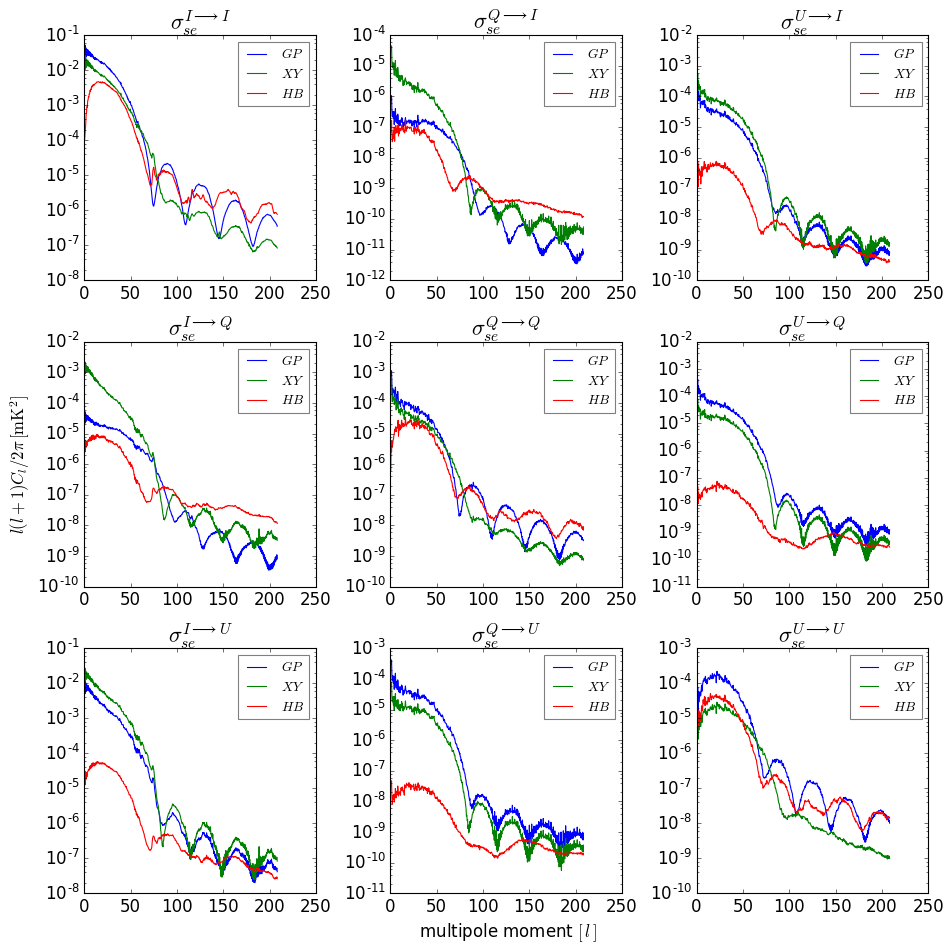
\includegraphics[width=6.6in]{powspectrum/osk_errplots}
%  \end{minipage}
%  \caption{\enquote{These are the spectra plots of the systematic errors as shown in Fig.~\ref{fig:fgerr}. 
%    The notations ${GP}$ and ${XY}$ in the legends denote the residuals for gain-phase and surface orientation errors in the OSKAR beams, 
%    that of ${HB}$ depicts the errors  in the holography beams. These errors are then used to estimate the imperfections in the simulation by 
%    computing the expected value of the standard deviations of the sampling distributions of the residual maps to produce Table~\ref{tbl:excel-table}.
%    } (Figure~\ref{fig:fg18} and the caption are obtained from \cite{ansah2018simulations})} \label{fig:fg18}.
%  \end{figure}
%  \FloatBarrier
%  %%


% % 
% \begin{table}\centering
% \caption{\enquote{Error introduced in the power spectrum estimation} (Table~\ref{tbl:excel-table} is reproduced from \cite{ansah2018simulations})} 
% \label{tbl:excel-table}
% % \ra{1.1}
% \begin{tabular}{@{}rrrcrrcrrcrr@{}}\toprule
% & \multicolumn{2}{c}{$\bm{I}$} & \phantom{abc}& \multicolumn{2}{c}{$\bm{Q}$} & \phantom{abc} & \multicolumn{2}{c}{$\bm{U}$} & \phantom{abc} & \multicolumn{2}{c}{$\bm{TOTAL}$}\\
% \cmidrule{2-3}  \cmidrule{5-6} \cmidrule{8-9} \cmidrule{11-12}
%  & $GP $ & $XY $ && $GP$ & $XY $  && $GP $ & $XY $  && $GP$ & $XY $ \\ \midrule
% % & GP $ & $ XY $ && $ GP  $ & $ XY $  && $ GP $ & $ XY $  && $ GP $ & $ XY $ \\ \midrule
% {}\\
% $\bm{I}$ & 0.0640 & 0.0640 && 0.0151 & 0.0137  && 0.0050 & 0.0045 && \textbf{0.0841} & \textbf{0.0822}\\
% $\bm{Q}$ & 0.0010 & 0.0008 && 0.0221 & 0.0224 && 0.0007 & 0.0055 && \textbf{0.0238} & \textbf{0.0287}\\
% $\bm{U}$ & 0.0007 & 0.0007 && 0.0194 & 0.0341 && 0.0354 & 0.0362  && \textbf{0.0555} & \textbf{0.0710}\\
% \bottomrule
% \end{tabular}
% %\caption{Caption}
% \end{table}
\end{appendices}
% \chapter{Software documentation}
% %st 1
% The following appendix serves as additional documentation for the installation and use of the {\sc meqsilhouette} simulator. Please reference \citep{Blecher_2016} when publishing results based on this code.
% 
% \section{Installation}
% %st 1
% 
% The {\sc meqsilhouette} repository is currently private, however if made public it is maintained here\footnote{https://github.com/ratt-ru/MeqSilhouette}. For bug reports, if public, open an issue on github/submit a pull request. Currently, the simulator is running on {\sc Ubuntu 14.04} and has not been tested on other operating systems. Software requirements which are being maintained elsewhere and are publicly available: 
% \begin{itemize}
%  \item {\sc simms}\footnote{https://github.com/radio-astro/simms}
%  \item {\sc MeqTrees}\footnote{https://ska-sa.github.io/meqtrees/} 
%  \item {\sc Scatterbrane}\footnote{http://krosenfeld.github.io/scatterbrane}
% \end{itemize}
% 
% Note that {\sc simms} in turn requires {\sc casa}, where we have had success with version 4.2.2. Several different routes for the installation of {\sc MeqTrees} are available\footnote{https://github.com/ska-sa/meqtrees/wiki/Installation}. As {\sc atm} is not currently being maintained or easily available, we include it within the {\sc meqsilhouette} repository. 
% 
% 
% Once the {\sc meqsilhouette} repository has been cloned, either add the framework module to the PYTHONPATH directly or install using pip,
% \begin{verbatim}
% $ cd MeqSilhouette/framework/; sudo pip install .
% \end{verbatim}
% \section{Usage}
% 
% %st 1
% We will first discuss the simple case of running a simulation with the canonical pre-written driver script. Following this, we will discuss how to write one's own driver script. We also list various miscellaneous notes which one should to be aware of when using {\sc meqsilhouette}.
% \subsection{Running a standard simulation}
% %st1
% 
% We will focus on the standard `azishe' pipeline, the central concepts are captured in Fig.~\ref{flow}, however antenna pointing errors are not included and the sky model needs to be in {\sc fits} format. 
% 
% To run in the MeqSilhouette repository we pass the driver script and parameter dictionary to {\sc Python},
% \begin{verbatim}
% $python driver/azishe.py input/parameters.json
% \end{verbatim}
% 
% 
% %Experimenting with parameters
% The content of the parameter dictionary is shown, slightly altered, in table~\ref{tab:parameters}. The parameters in the dictionary can be edited directly. 
% 
% %logging
% The primary log is set by `v.LOG' variable, initialised in the driver script. If the variable is commented out, the logs will display to screen. 
% 
% %Outputs
% The output directory is set by the `v.OUTPUT' variable, initialised in the driver script. In this directory there will be a variety of files, a list and explanation of which is given in table~\ref{tab:outputs}.
% 
% \begin{longtable}{p{0.5\linewidth}|p{0.5\linewidth}}
% \caption[List and explanation of files output by a standard simulation]{List and explanation of files output by a standard simulation. There are several file formats and data types in parenthesis for easier comprehension. (antenna-based) {\sc NumPy} arrays have a shape corresponding to indexing (Time, Frequency, Antenna); ({\sc ms}-structured) {\sc NumPy} arrays reflect the data format of the {\sc ms} (i.e. Row, Frequency, Polarisation); (baseline dictionary) refers to {\sc pickle} dictionaries where keys are (Station 1, Station 2); (triangle dictionary) is same as a (baseline dictionary) except with an extra dimension i.e. (Station 1, Station 2, Station 3).}
% \label{tab:outputs}\\
% \hline
% name&comment\nl
% \hline
% measurement set (.MS) & simulated Measurement set \nl
% sky models (.fits)& sky models which were observed\nl
% parameters (.json) &input parameter dictionary\nl
% (atm/antenna number)atm abs (.txt)& zenith atmospheric opacity and sky brightness temperature output by {\sc atm}\nl
% (atm/antenna number)atm disp (.txt)& zenith atmospheric delays output by {\sc atm}\nl
% closure phases (.p) & Dictionary of closure phases  (triangle dictionary)\nl
% closure phase uncertainties (.p) & Dictionary of closure phase uncertainties (triangle dictionary)\nl
% Thermal noise  (.p)  & Dictionary of expected thermal noise levels used to generate closure phase uncertainties (baseline dictionary)\nl
% SNR (.p)  & Dictionary of SNR values (see equation~\ref{eq:snr}) used to generate closure phase uncertainties (baseline dictionary). \nl
% receiver noise (.npy) & thermal noise generated from $SEFD$s ({\sc ms}-structured)\nl
% sky noise (.npy) & thermal noise generated from atmosphere ({\sc ms}-structured)\nl
% transmission (.npy) & atmosphere transmission (antenna-based)\nl
% turbulent phases (.npy) & atmospheric phase terms (antenna-based)\nl
% Stokes I (.p)& visibilities in total intensity (baseline dictionary)\nl
% phase standard deviations (.npy)& standard deviations of the phase error between two data points at zenith (antenna-based)\nl
% turbulent phases (.npy) & turbulent contribution to the atmospheric phase error (antenna-based)\nl
% phase normalisation (.npy) & mean contribution to atmospheric phase error (antenna-based)\nl
% 
% 
% \end{longtable}
% 
% \subsubsection{Further notes and reminders}
% \begin{itemize}
%  \item If the content of antenna table is changed, so should the content of station information file, which contains station $SEFD$ and weather information. 
%  \item Ensure that the order of stations in the station information file matches the order in the antenna table.
%  \item Ensure that the antenna table is complete, including names, positions in metres and dish diameters.
%  \item Ensure that the {\sc fits} file is complete with satisfactory header and data shape (see examples in the input directory for guidance).
%  \item Currently one spectral window can be simulated at a time.
%  \item Currently only total intensity (RR and LL components) are simulated, see section~\ref{sec:full_stokes} for more information.
%  \item There are several cautions related to usage of {\sc scatterbrane}, including a restriction on the compactness of sky models. See original documentation \footnote{http://krosenfeld.github.io/scatterbrane/current/}. 
%  \item The path of the folder containing the sky model is also located in the parameter dictionary, for multiple fits files, i.e. a time-variable source, the order of their implementation is the same as if their names with sorted with numpy.sort, where each fits files is observed for approximately the same amount of time. If the ISM-scattering is turned on, the extra logistics of moving and creating fits files and folders are automatically handled.
% \end{itemize}
% 
% \subsection{Writing a driver script}
%  
% Often it is useful to perform iterations of subset of steps of the standard pipeline which is straightforward with a \emph{for} loop and several simple functions or clearing and copying measurement sets. A number of different pipelines are available in the driver scripts folder, which should be provide `worked examples' when writing a novel driver script. The most important steps are:
% \begin{enumerate}
%  \item setup parameter dictionary as well as sub-dictionaries
%  \item create measurement set
%  \item initialise SimCoordinator class
%  \item Use SimCoordinator to generate visibilities and apply signal corruptions
% \end{enumerate}
% 
%  Also, it is also possible to save/load from most of the signal corruptions if you needed to ensure that the corruption used is exactly the same in different realisations. 
% 
% 
% 
% If additional instrumental corruptions are implemented, this should be within the TropMS class for consistency. Also it is important that the pipeline respects the causality of signal transmission path and/or the commutativity of Jones-matrices.
% 
% 
















